
\documentclass[aspectratio=169]{beamer}

\usetheme{Madrid}
\usecolortheme{seahorse}

\usepackage[utf8]{inputenc}
\usepackage{amsmath, amsfonts, amssymb}
\usepackage{booktabs}
\usepackage{array}
\usepackage{tikz}
\usepackage{ragged2e}

\definecolor{AccentBlue}{RGB}{0,92,184}
\setbeamercolor{structure}{fg=AccentBlue}
\setbeamercolor{title}{fg=white,bg=AccentBlue}
\setbeamercolor{frametitle}{fg=AccentBlue}
\setbeamercolor{block title}{bg=AccentBlue!10, fg=black}
\setbeamercolor{block body}{bg=gray!5, fg=black}

\setbeamertemplate{navigation symbols}{}

% --- Placeholder macro for figures/diagrams ---
\newcommand{\figplaceholder}[1]{%
  \begin{center}
    \begin{tikzpicture}
      \draw[gray!70, dashed] (0,0) rectangle (11.5,5.2);
      \node[align=center, text width=11cm] at (5.75,2.6) {\Large \textbf{Figure Placeholder}\\[0.4em]\normalsize #1};
    \end{tikzpicture}
  \end{center}
}

% --- Section intro slide ---
\newcommand{\sectionintro}[1]{%
  \begin{frame}[plain]
  \transfade
  \vfill
  \begin{center}
    {\LARGE \color{AccentBlue}\textbf{#1}}
  \end{center}
  \vfill
  \end{frame}
}

\title[Contemporary Economic Issues]{Income Inequality and Poverty}
\subtitle{ECON 204 -- Contemporary Economic Issues}
\author{Muhebullah Karimzada}
%\institute{Winter 2026}
\date{Winter 2026}

\begin{document}

\begin{frame}
\transfade
\titlepage
\end{frame}



\begin{frame}{Learning Objectives}
\transfade
\begin{itemize}[<+->]
\item How to define and measure \textbf{income inequality} and \textbf{poverty}.
\item How to analyze the evolution of inequality and poverty by individual characteristics in \textbf{Canada}.
\item How to compare Canada with other countries.
\item How to analyze the comovement between inequality, poverty, and \textbf{real per capita GDP}.
\end{itemize}
\end{frame}

\begin{frame}{Key terms (1/3)}
\transfade
\begin{itemize}[<+->]
\item \textbf{Decile:} When the population is divided into ten equal groups ordered with respect to a variable, the groups are called deciles. For example, the first income decile is one tenth (10\%) of the population with the lowest income.\\

\item \textbf{Economic growth:} This is the growth rate of the real per capita GDP.\\

\item \textbf{Economic mobility:} This characterizes the ability for individuals to move from one part of the income distribution to another.\\

\item \textbf{Gini coefficient:} This is a global measure of inequality. It goes from 0 (perfect equality) to 1 (perfect inequality).
\end{itemize}
\end{frame}

\begin{frame}{Key terms (2/3)}
\transfade
\begin{itemize}[<+->]
\item \textbf{Income share:} This is the proportion of total income that goes to an individual or a group. For example, if the income share of females is 55\%, it means that 55\% of the total income is earned by women.
\item \textbf{Lorenz curve:} This is a line chart that illustrates the cumulative income share of the population as a function of the proportion of the population.
\item \textbf{Low income measure (LIM):} This is equal to half the median of income. It is one of the measures of the poverty line. Individuals with income less than the LIM are considered below the poverty line.

\end{itemize}
\end{frame}


\begin{frame}{Key terms (3/3)}
\transfade
\begin{itemize}[<+->]

\item \textbf{Market basket measure (MBM):} This is the value of a basket of goods used in one definition of the poverty line. Individuals with income less than the MBM are considered below the poverty line.
\item \textbf{Median:} This is a number that separates the distribution of a variable in two equal groups.
\item \textbf{Per capita:} This is a Latin word that means ``by head''.
\item \textbf{Quintile:} When the population is divided into five equal groups ordered with respect to a variable, the groups are called quintiles.
\end{itemize}
\end{frame}




\begin{frame}{Economic growth}
\transfade
\begin{itemize}[<+->]
\item Economic growth is defined as the growth rate of the \textbf{real per capita GDP} defined as
\[
\text{Real per capita GDP} = \frac{\text{Real GDP}}{\text{Population}}.
\]
\item Since GDP is also a measure of total income, we also call it \textbf{average real per capita income}.
\item To obtain real per capita GDP, download:
\begin{itemize}[<+->]
\item the real GDP series and
\item the population series.
\end{itemize}
\item Be careful with units: population is in \emph{units} and GDP is in \emph{millions}; express population in millions before dividing.
\end{itemize}
\end{frame}

\begin{frame}{Real per capita GDP and its growth (illustrations)}
\transfade

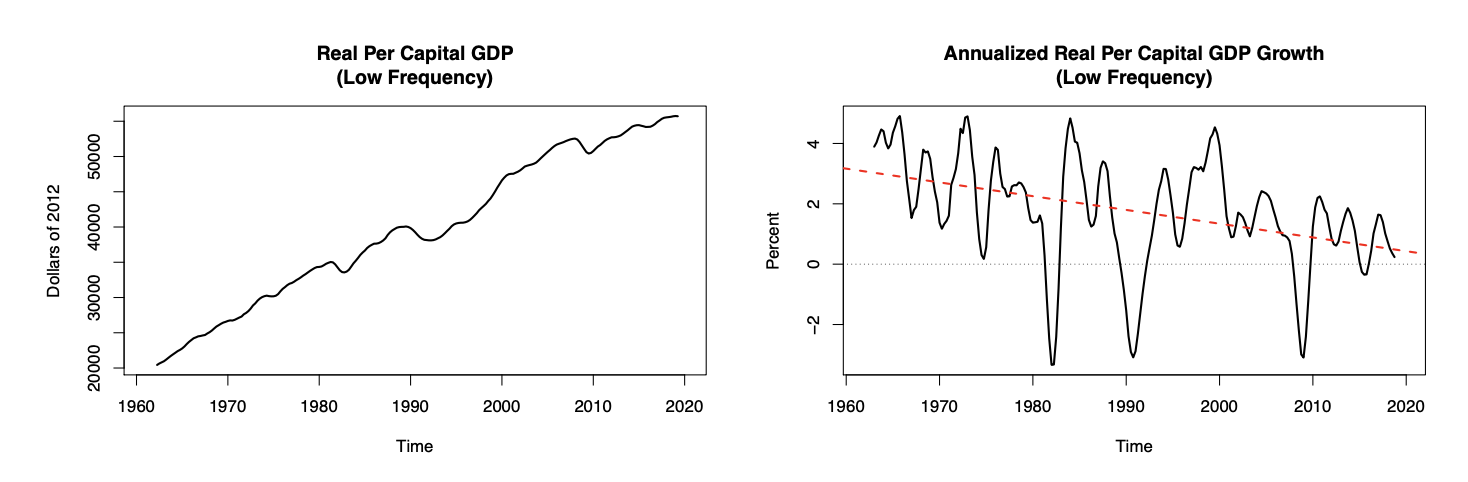
\includegraphics[width=0.85\linewidth]{Fig1}.
\begin{itemize}

 \item Low-frequency component of real per capita GDP (left) and annualized low-frequency real per capita GDP growth (right).
 \item Real per capita GDP rises from about \$20{,}000 to about \$55{,}000 (2012 dollars) between 1961 and 2020; growth rate declines on average.
 \end{itemize}
\end{frame}

\begin{frame}{Why growth is not enough}
\transfade
\begin{itemize}[<+->]
\item The rise in real per capita GDP implies Canadians get richer on average and standards of living improve on average.
\item But it does \textbf{not} imply that the standard of living of \emph{every} Canadian has improved.
\item This lecture focuses on the \textbf{allocation} of real GDP/income across individuals, how it evolves, and how it relates to growth.
\end{itemize}
\end{frame}

\begin{frame}{Quintiles: idea and construction}
\transfade
\begin{itemize}[<+->]
\item Quintiles divide the population into five equal groups (20\% each), ordered by the variable of interest.
\item The lowest quintile contains the 20\% with the smallest values; the fifth quintile contains the 20\% with the highest values.
\item Which individuals fall into each quintile depends on the variable used (e.g., age vs expenditure).
\end{itemize}
\end{frame}

\begin{frame}{Expenditure and age by individual}
\transfade
\begin{center}
\scriptsize
\setlength{\tabcolsep}{1pt}
\renewcommand{\arraystretch}{1.1}
\begin{tabular}{p{0.20\linewidth}*{15}{>{\centering\arraybackslash}p{0.05\linewidth}}}
\toprule
\textbf{Individual} & 1 & 2 & 3 & 4 & 5 & 6 & 7 & 8 & 9 & 10 & 11 & 12 & 13 & 14 & 15 \\
\midrule
\textbf{Age} & 19 & 23 & 45 & 18 & 64 & 55 & 34 & 23 & 22 & 44 & 70 & 61 & 49 & 21 & 43 \\
\textbf{Expenditure} & 100 & 210 & 80 & 30 & 312 & 190 & 201 & 236 & 341 & 34 & 40 & 101 & 170 & 190 & 343 \\
\bottomrule
\end{tabular}
\end{center}
\end{frame}

\begin{frame}{Age quintiles (sorted by age)}
\transfade
\begin{center}
\scriptsize
\setlength{\tabcolsep}{2pt}
\renewcommand{\arraystretch}{1.1}
\begin{tabular}{p{0.24\linewidth} p{0.152\linewidth} p{0.152\linewidth} p{0.152\linewidth} p{0.152\linewidth} p{0.152\linewidth}}
\toprule
& \textbf{First} & \textbf{Second} & \textbf{Third} & \textbf{Fourth} & \textbf{Fifth} \\
\midrule
\textbf{Individuals} & 4, 1, 14 & 9, 2, 8 & 7, 15, 10 & 3, 13, 6 & 12, 5, 11 \\
\textbf{Age} & 18, 19, 21 & 22, 23, 23 & 34, 43, 44 & 45, 49, 55 & 61, 64, 70 \\
\textbf{Expenditure} & 30, 100, 190 & 341, 210, 236 & 201, 343, 34 & 80, 170, 190 & 101, 312, 40 \\
\bottomrule
\end{tabular}
\end{center}
\end{frame}

\begin{frame}{Measuring inequality: income by quintile}
\transfade
\begin{itemize}[<+->]
\item A simple way to summarize inequality is to compare the \textbf{average income} across quintiles and the \textbf{share of total income} held by each quintile.
\item If higher-income quintiles capture a much larger income share, the distribution is more unequal.
\end{itemize}
\end{frame}

\begin{frame}{Average income by quintile in 2018}
\transfade
\begin{center}
\small
\begin{tabular}{p{0.3\linewidth} p{0.30\linewidth} p{0.28\linewidth}}
\toprule
\textbf{Quintile} & \textbf{Average Household Income (dollars)} & \textbf{Share of Total Household Income (\%)} \\
\midrule
First Income Quintile & 23{,}537 & 5.90 \\
Second Income Quintile & 49{,}137 & 12.40 \\
Third Income Quintile & 69{,}943 & 17.60 \\
Fourth Income Quintile & 91{,}798 & 23.10 \\
Fifth Income Quintile & 162{,}231 & 40.90 \\
\bottomrule
\end{tabular}
\end{center}
\end{frame}

\begin{frame}{Cumulative income share in Canada in 2018}
\transfade
\begin{itemize}[<+->]
\item The cumulative share of income is the share of income of the first quintile (bottom 20\%), the first two quintiles (bottom 40\%), the first three (bottom 60\%), and so on.
\end{itemize}
\begin{center}
\small
\begin{tabular}{p{0.55\linewidth} p{0.35\linewidth}}
\toprule
\textbf{Group} & \textbf{Cumulative Income Share (\%)} \\
\midrule
The bottom 20\% & 5.90 \\
The bottom 40\% & 18.30 \\
The bottom 60\% & 35.90 \\
The bottom 80\% & 59.00 \\
The bottom 100\% & 99.90 \\
\bottomrule
\end{tabular}
\end{center}
\end{frame}

\begin{frame}{Lorenz curve}
\transfade
\begin{itemize}[<+->]
\item The Lorenz curve plots cumulative income share (y-axis) as a function of cumulative households (x-axis).
\item Perfect equality implies: bottom 20\% gets 20\%, bottom 40\% gets 40\%, etc. (the 45-degree equality line).
\item The farther the Lorenz curve is from the equality line, the more unequal the distribution.
\end{itemize}
\end{frame}

\begin{frame}{Lorenz curve: Canada (2018) and USA (2009)}

\center
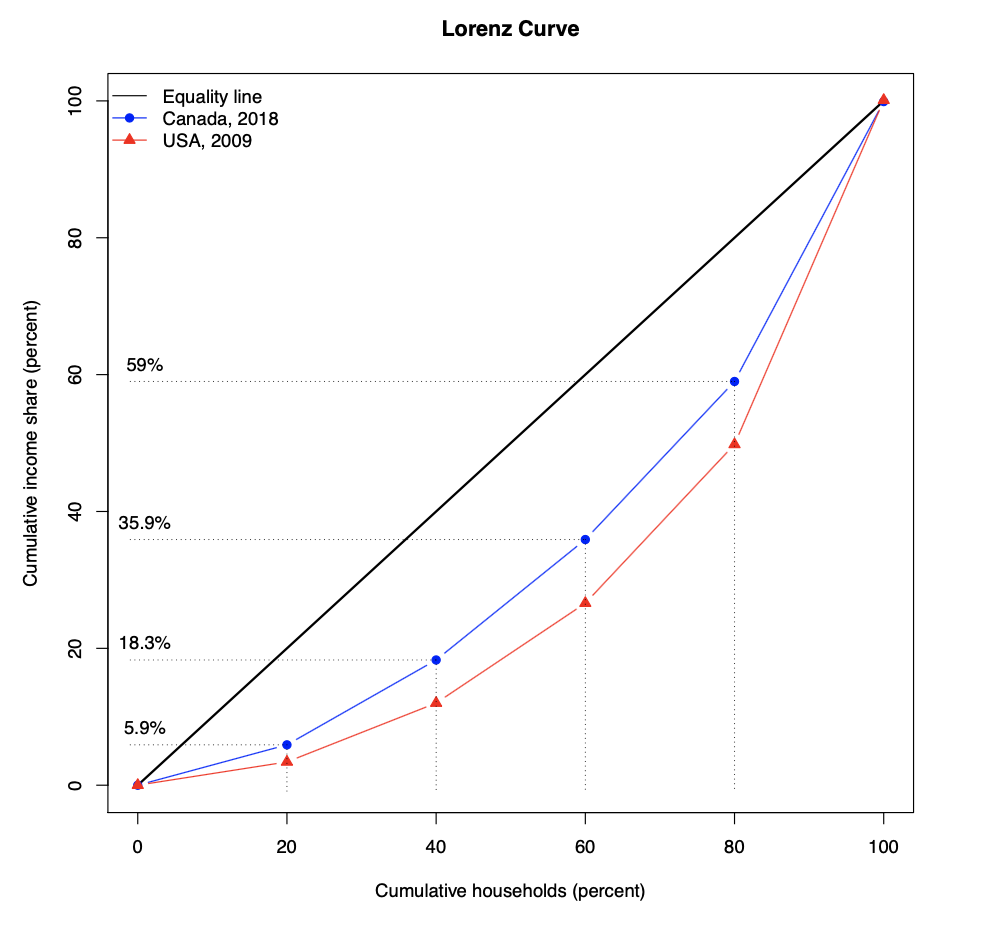
\includegraphics[width=0.55\linewidth]{Fig2}.

\end{frame}



\begin{frame}{Lorenz curve: Canada (2018) and USA (2009)}
\transfade

\begin{itemize}[<+->]
\item Lorenz curve with equality line.   \item Coordinates shown for Canada: 5.9\%, 18.3\%, 35.9\%,  and 59\%.
\item Conclusion: USA (2009) allocation is more unequal than Canada (2018).
\end{itemize}
\end{frame}

\begin{frame}{The Gini coefficient}
\transfade
\begin{itemize}[<+->]
\item The Gini coefficient is based on the Lorenz curve.
\item It is the area between the equality line and the Lorenz curve divided by the area under the equality line.
\item The area under the equality line is $0.5$, so the Gini coefficient is \textbf{twice} the area between the two curves.
\item It equals 0 when the Lorenz curve is the equality line, and increases as inequality rises.
\end{itemize}
\end{frame}

\begin{frame}{Gini coefficient with quintiles}
\transfade
\begin{itemize}[<+->]
\item Let $h_i=(i/5-s_i)$ for $i=1,2,3,4$, be the distance between the equality line and the Lorenz curve at 20\%, 40\%, 60\% and 80\%, where $s_i$ is the cumulative income share of quintiles 1 to $i$.
\item Then the Gini coefficient is:
\[
\text{Gini} = 0.40 \times (h_1+h_2+h_3+h_4) = 0.8-0.4\times(s_1+s_2+s_3+s_4).
\]
\item With quintiles, the maximum Gini is $0.8$ (to reach 1, we need more than 5 groups).
\end{itemize}
\end{frame}

\begin{frame}{Background: geometry intuition}
\transfade
\begin{itemize}[<+->]
\item Between two adjacent points on the Lorenz curve, the area between the Lorenz curve and the equality line is a trapezoid.
\item If the trapezoid has bases $a$ and $b$ and height $c$, its area is $(a+b)\,c/2$.
\item In our setup: $a$ and $b$ are successive distances ($h_i$'s), and $c=0.20$ (20\% of the population).
\item Add trapezoid areas across segments and multiply by 2 to get the Gini coefficient.
\end{itemize}
\end{frame}

\begin{frame}{Gini coefficient in general (n groups)}
\transfade
\begin{itemize}[<+->]
\item If we split the population into $n$ equal groups, define $h_i=(i/n-s_i)$ for $i=1,\dots,n-1$, where $s_i$ is the cumulative income share of groups 1 to $i$.
\item Then:
\[
\text{Gini}=\frac{2}{n}\sum_{i=1}^{n-1} h_i.
\]
\item Replacing $h_i$ by $i/n-s_i$ yields:
\[
\text{Gini}=\frac{n-1}{n}-\frac{2}{n}\sum_{i=1}^{n-1} s_i.
\]
\item The maximum is $(n-1)/n$, which approaches 1 as $n$ becomes large.
\end{itemize}
\end{frame}

\begin{frame}{Lorenz curve: individual vs household}
\transfade
\center

\includegraphics[width=0.47\linewidth]{Fig3}.
\begin{footnotesize}
\begin{itemize}
\item Lorenz curve at individual level (2016) and household level (2018), with equality line.
\item More groups $\Rightarrow$ smoother curve; inequality is higher at the individual level.
\end{itemize}
\end{footnotesize}
\end{frame}

\begin{frame}{The evolution of the Gini coefficient in Canada}
\transfade
\begin{itemize}[<+->]
\item Statistics Canada publishes an annual series of the Gini coefficient starting in 1976.
\item The Gini coefficient is based on \textbf{household income adjusted for family size}, using adjusted after-tax income (income from all sources including government transfers less income tax).
\item It was roughly constant from 1976 to the end of the 1980s, increased from the early 1990s to the early 2000s, then decreased onward.
\item The business cycle affects inequality (e.g., increases during recessions of 1982 and 1990).
\end{itemize}
\end{frame}

\begin{frame}{Gini coefficient in Canada}
\transfade
\center
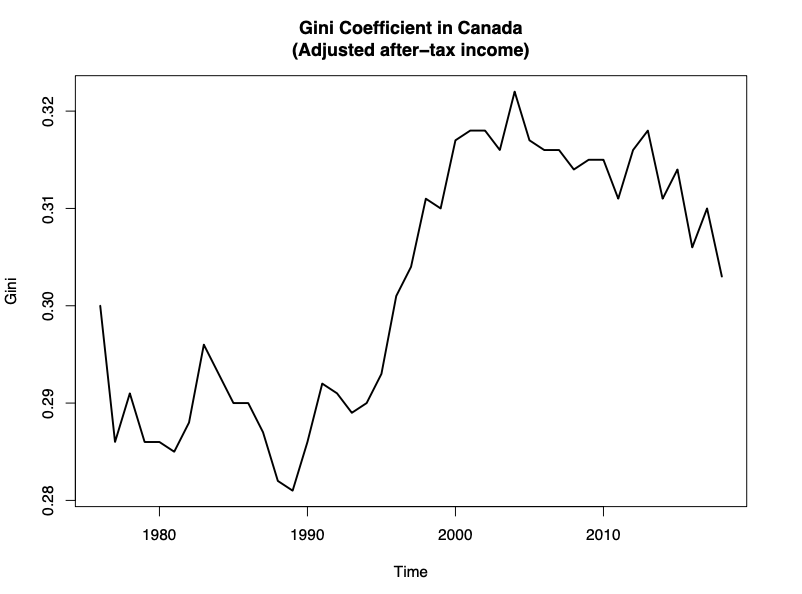
\includegraphics[width=0.5\linewidth]{Fig4}.
\begin{itemize}


\item Time series: Gini coefficient in Canada (adjusted after-tax income), 1976--2018. \item Stable through late 1980s; rises in early 1990s to early 2000s; then declines.
\end{itemize}
\end{frame}

\begin{frame}{Gini coefficient in some provinces}
\transfade
\begin{itemize}[<+->]
\item Ontario is the province where inequality increased the most over the period; by 2018, New Brunswick and Quebec had the least inequality among the four shown.
\end{itemize}
\center
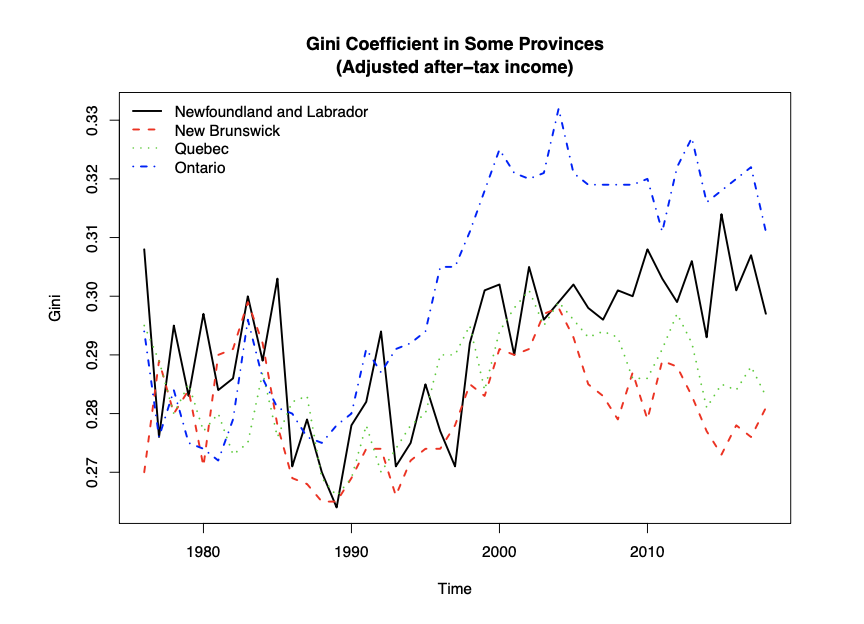
\includegraphics[width=0.48\linewidth]{Fig5}.
\begin{itemize}

\item Gini coefficient (adjusted after-tax income) for Newfoundland and Labrador, New Brunswick, Quebec, Ontario.

\end{itemize}
\end{frame}

\begin{frame}{Comparing the Gini coefficient across countries}
\transfade
\begin{itemize}
\item To compare across countries, coefficients should come from the \textbf{same source} and be computed consistently.
\item A bar chart for 2015 shows Canada in the middle among the shown countries; the United States is among the most unequal; Slovakia is among the most equal; South Africa is the most unequal in the chart.
\end{itemize}

\end{frame}


\begin{frame}{Comparing the Gini coefficient across countries}

\center
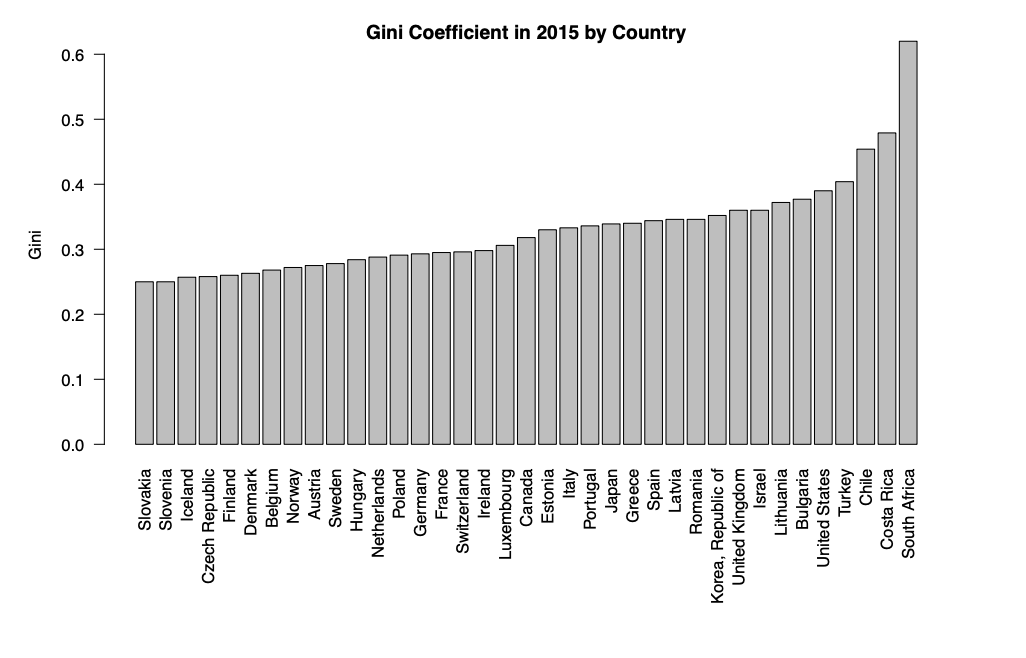
\includegraphics[width=0.68\linewidth]{Fig6}.
\begin{itemize}


\item Bar chart: Gini coefficient in 2015 by country (selected OECD/non-OECD).
\end{itemize}
\end{frame}

\begin{frame}{Exercises: measuring the Gini coefficient}
\transfade
\begin{itemize}[<+->]
\item \textbf{1.} Consider the following table of average income by quintile. Compute the Gini coefficient.
\end{itemize}
\begin{center}
\small
\begin{tabular}{p{0.60\linewidth} p{0.30\linewidth}}
\toprule
\textbf{Quintile} & \textbf{Average Income (dollars)} \\
\midrule
First Income Quintile & 342 \\
Second Income Quintile & 642 \\
Third Income Quintile & 844 \\
Fourth Income Quintile & 990 \\
Fifth Income Quintile & 1{,}053 \\
\bottomrule
\end{tabular}
\end{center}
\end{frame}

\begin{frame}{Exercises: measuring the Gini coefficient (continued)}
\transfade
\begin{itemize}[<+->]
\item \textbf{2.} Consider the following table of average income by decile. Compute the Gini coefficient.
\end{itemize}
\begin{center}
\small
\begin{tabular}{p{0.60\linewidth} p{0.30\linewidth}}
\toprule
\textbf{Decile} & \textbf{Average Income (dollars)} \\
\midrule
First Income Decile & 114 \\
Second Income Decile & 288 \\
Third Income Decile & 605 \\
Fourth Income Decile & 621 \\
Fifth Income Decile & 1{,}012 \\
Sixth Income Decile & 1{,}023 \\
Seventh Income Decile & 1{,}101 \\
Eighth Income Decile & 1{,}434 \\
Nineth Income Decile & 1{,}925 \\
Tenth Income Decile & 1{,}934 \\
\bottomrule
\end{tabular}
\end{center}
\end{frame}

\begin{frame}{Exercise solution (deciles): shares and cumulative shares}
\transfade
\begin{itemize}[<+->]
\item Income share of decile $i$ is average income in decile $i$ divided by the sum of average incomes.
\item Example: for the first decile,
\[
S_1=\frac{114}{114+288+605+621+1{,}012+1{,}023+1{,}101+1{,}434+1{,}925+1{,}934}=1.13\%.
\]
\item Compute cumulative shares, then apply the general formula with $n=10$:
\[
\text{Gini}=\frac{n-1}{n}-\frac{2}{n}(s_1+s_2+\cdots+s_9).
\]
\end{itemize}
\end{frame}

\begin{frame}{Decile shares table (rounded at the end)}
\transfade
\begin{center}
\small
\begin{tabular}{p{0.42\linewidth} p{0.18\linewidth} p{0.18\linewidth} p{0.18\linewidth}}
\toprule
\textbf{Decile} & \textbf{Avg. Income} & \textbf{Income share (\%)} & \textbf{Cumulative shares (\%)} \\
\midrule
First Income Decile & 114 & 1.13 & 1.13 \\
Second Income Decile & 288 & 2.86 & 4.00 \\
Third Income Decile & 605 & 6.02 & 10.01 \\
Fourth Income Decile & 621 & 6.17 & 16.19 \\
Fifth Income Decile & 1{,}012 & 10.06 & 26.25 \\
Sixth Income Decile & 1{,}023 & 10.17 & 36.42 \\
Seventh Income Decile & 1{,}101 & 10.95 & 47.37 \\
Eighth Income Decile & 1{,}434 & 14.26 & 61.63 \\
Nineth Income Decile & 1{,}925 & 19.14 & 80.77 \\
Tenth Income Decile & 1{,}934 & 19.23 & 100.00 \\
\bottomrule
\end{tabular}
\end{center}
\end{frame}

\begin{frame}{Measure of poverty}
\transfade
\begin{itemize}[<+->]
\item Income inequality is particularly problematic when it implies that a large proportion of the population is in a state of poverty.
\item An household is considered poor if its income falls below the \textbf{poverty line}.
\item Two measures used by Statistics Canada:
\begin{itemize}[<+->]
\item the \textbf{market basket measure (MBM)}, and
\item the \textbf{low income measure (LIM)}.
\end{itemize}
\end{itemize}
\end{frame}

\begin{frame}{The market basket measure (MBM)}
\transfade
\begin{block}{Definition}
The Market Basket Measure (MBM) is based on the cost of a specific basket of goods and services representing a modest, basic standard of living. It includes the costs of food, clothing, shelter, transportation and other items for a reference family. These costs are compared to the disposable income of families to determine whether or not they fall below the poverty line.
\end{block}
\begin{itemize}[<+->]
\item A household is below the poverty line if it cannot afford the ``modest and basic standard of living'' determined by the basket.
\item The table includes the proportion of persons below the poverty line by characteristics starting in 2006.
\end{itemize}
\end{frame}

\begin{frame}{Proportion below poverty line in 2018 (MBM)}
\transfade
\center
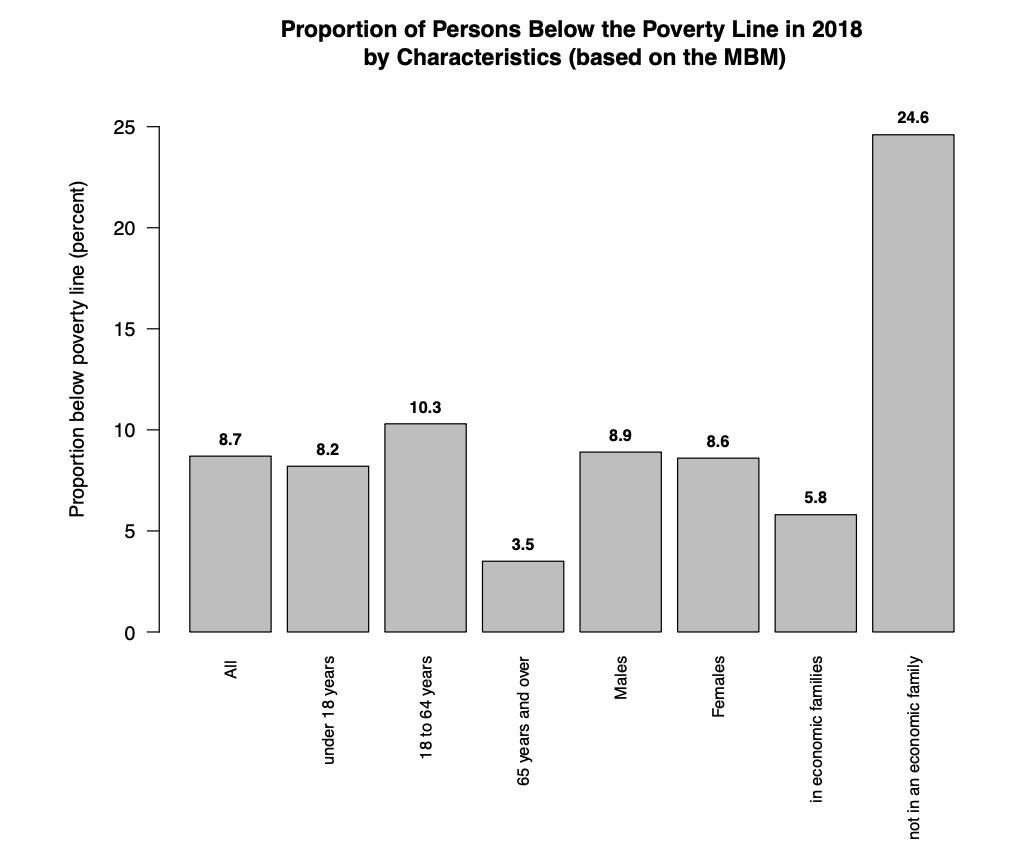
\includegraphics[width=0.58\linewidth]{Fig7}.

\end{frame}

\begin{frame}{The low income measure (LIM)}
\transfade
\begin{itemize}[<+->]
\item Another definition of poverty line is the low income measure (LIM).
\item It is equal to half the adjusted median household income (adjusted for household size).
\item Median household income in 2018 was \$61,400, so households with income less than \$30,700 are below the poverty line (before adjusting for household size).
\item The LIM series is based on adjusted after-tax income.
\end{itemize}
\end{frame}

\begin{frame}{Proportion below poverty line in 2018 (LIM)}
\center
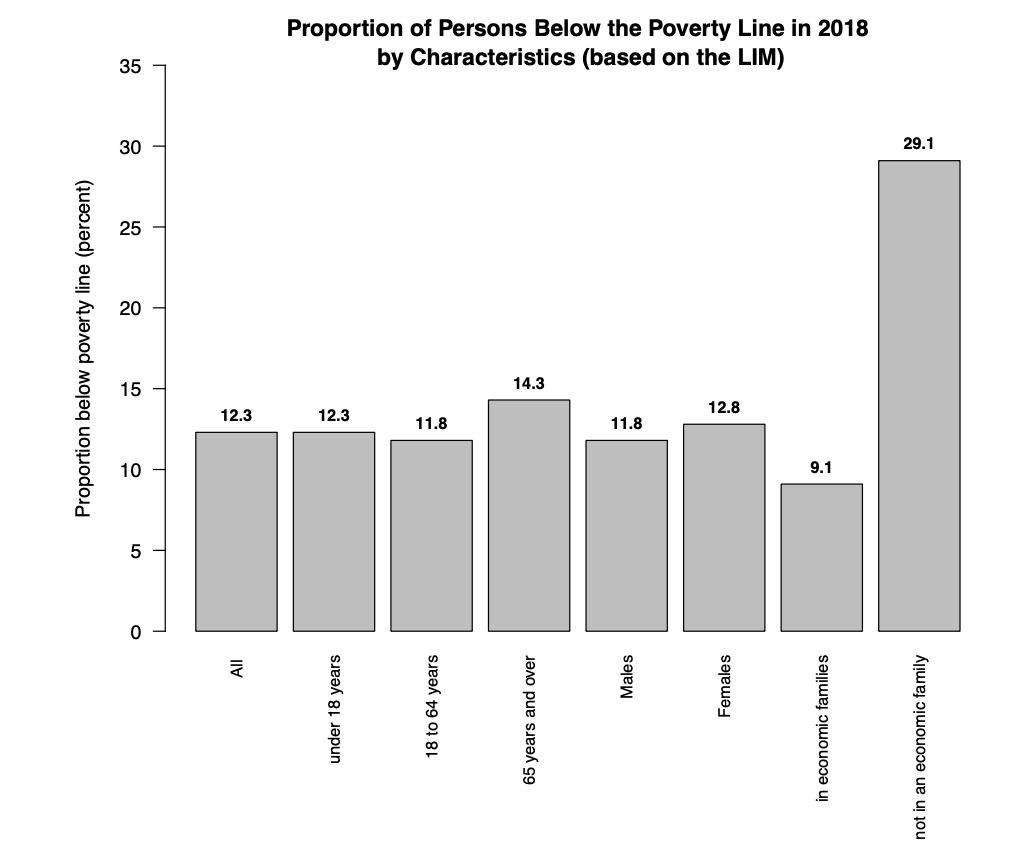
\includegraphics[width=0.58\linewidth]{Fig8}.
\end{frame}

\begin{frame}{Poverty over time in Canada (LIM)}
\transfade
\begin{itemize}[<+->]
\item Evolution of poverty from 1976 to 2018 based on LIM.
\item Left graph: all persons, males, females, persons in economic families.
\item Right graph: all persons not in family, males not in family, females not in family.
\item Overall: poverty decreased from 1976 to 1990 and increased after 1990; persons in family were quite stable.
\item Females were systematically more likely to be below the poverty line than males, but the gap narrowed by 2018.
\end{itemize}
\end{frame}

\begin{frame}{Poverty over time }
\center
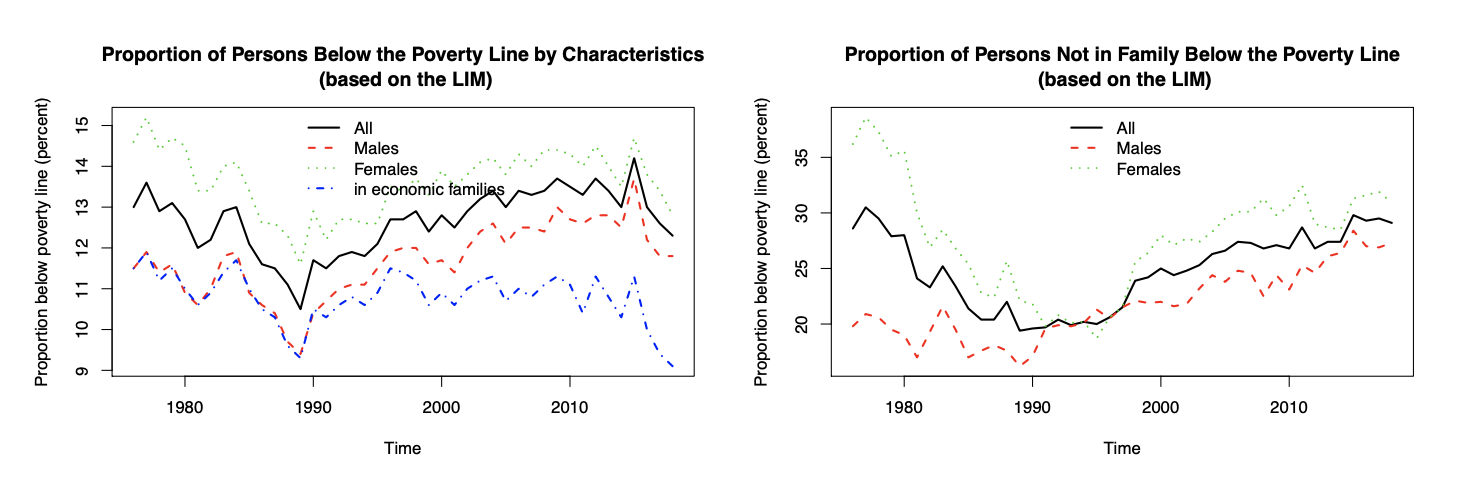
\includegraphics[width=0.98\linewidth]{Fig9}.
\end{frame}

\begin{frame}{Important: poverty vs inequality}
\transfade
\begin{itemize}[<+->]
\item Is poverty related to inequality? \textbf{Not necessarily.}
\item Everyone could be poor $\Rightarrow$ poverty high but inequality low.
\item Everyone could be above the poverty line $\Rightarrow$ poverty low but inequality could still be high.
\item Poverty focuses on the bottom of the distribution; inequality focuses on dispersion across the whole distribution.
\end{itemize}
\end{frame}



\begin{frame}{Exercise: poverty versus per capita GDP in Canada}
\transfade
\begin{itemize}[<+->]
\item You need:
\begin{itemize}[<+->]
\item proportion of persons below the poverty line (LIM) by characteristics,
\item annual real GDP series, and
\item annual population series.
\end{itemize}
\item Analyze the relationship between poverty and real per capita GDP by characteristics.
\item Use scatter plots and compare:
\begin{itemize}[<+->]
\item males vs females,
\item males vs females in economic families,
\item males vs females not in economic families.
\end{itemize}
\end{itemize}
\end{frame}

\begin{frame}{Exercise solution: scatter plots}
\center
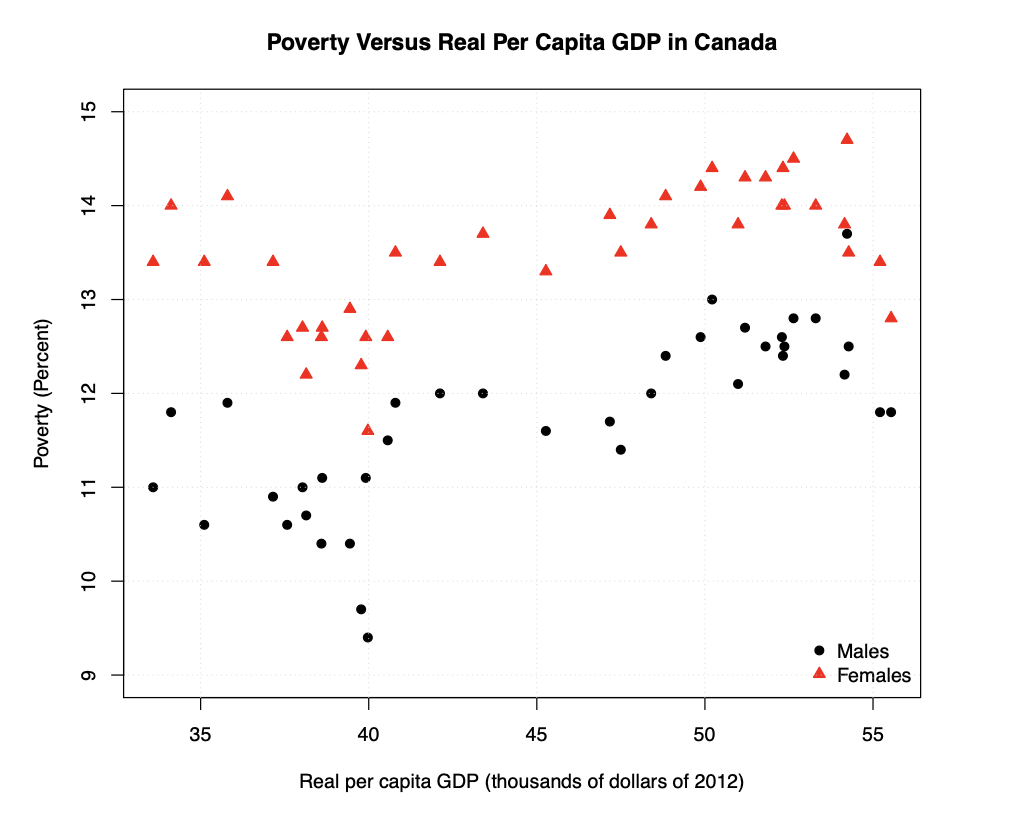
\includegraphics[width=0.58\linewidth]{Fig10}.
\end{frame}

\begin{frame}{Poverty vs GDP: persons in economic families}
\center
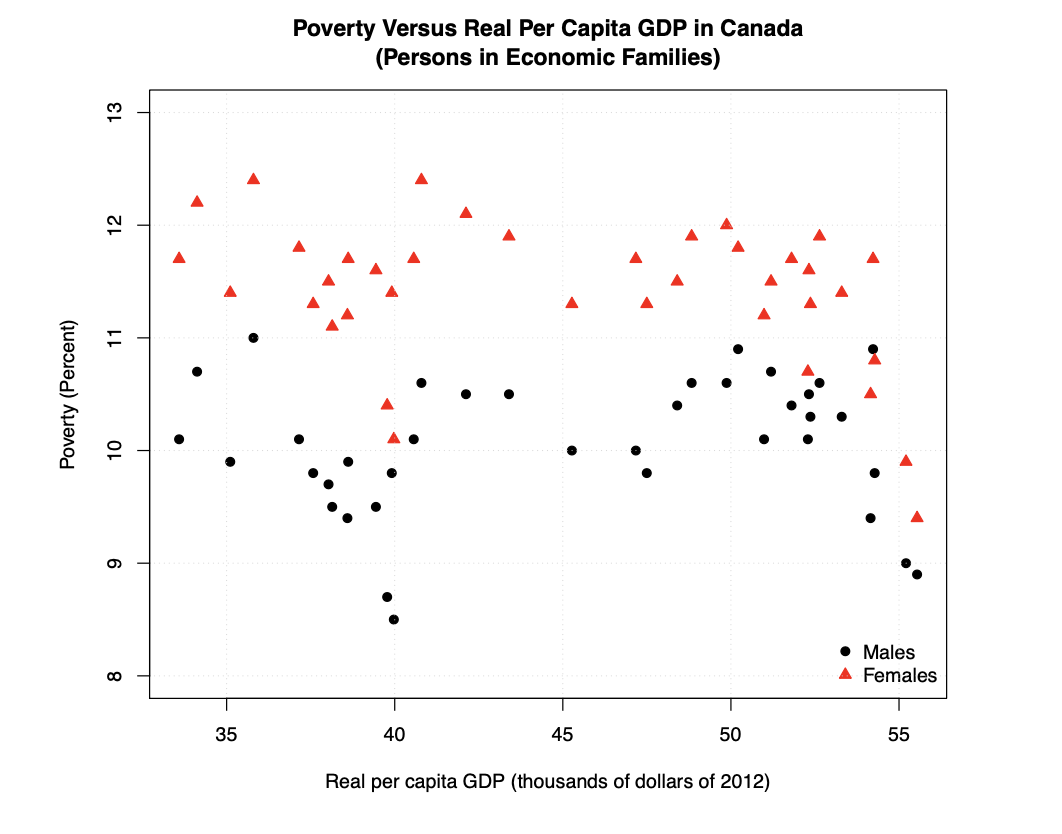
\includegraphics[width=0.58\linewidth]{Fig11}.
\end{frame}

\begin{frame}{Poverty vs GDP: persons not in economic families}
\center
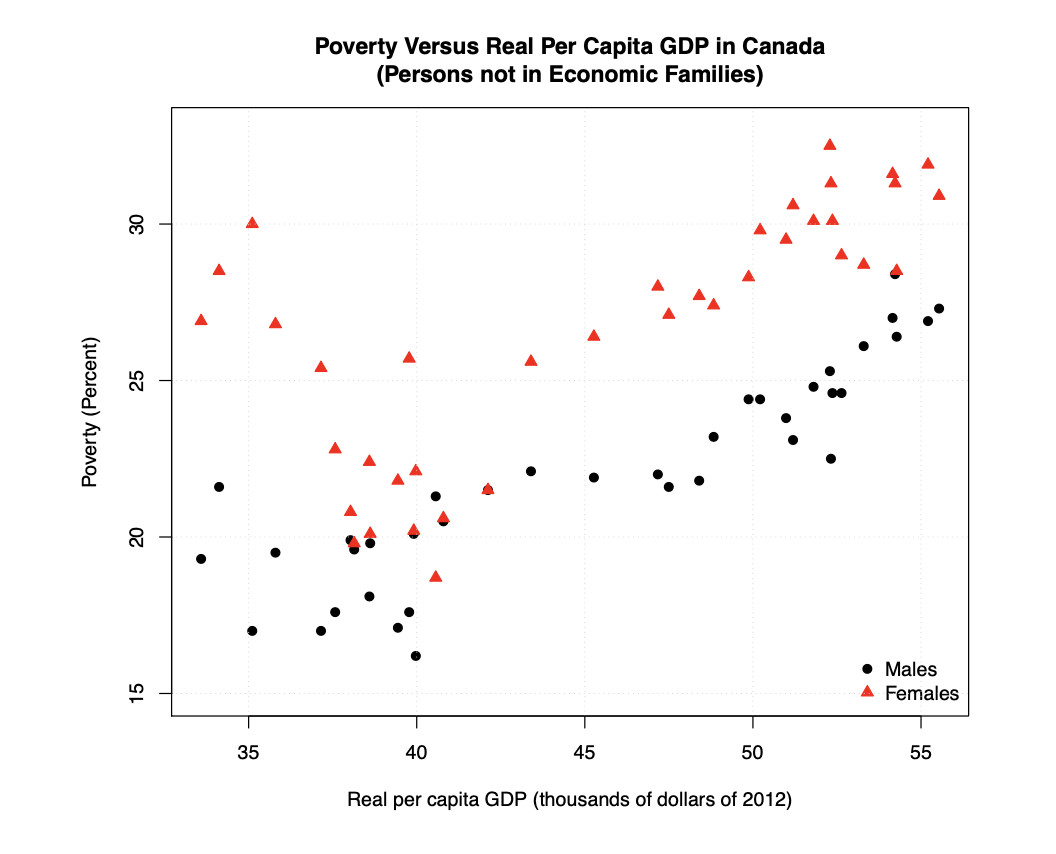
\includegraphics[width=0.58\linewidth]{Fig12}.
\end{frame}



\begin{frame}{Sources of inequality}
\transfade
\begin{itemize}[<+->]
\item \textbf{Inequality in skills:} Highly demanded skills command higher pay (e.g., skilled NHL hockey players; coding skills).
\item \textbf{Inequality in how skills are valued:} Income differences depend on how society values goods/services and on demand vs supply of skills.
\item \textbf{Inequality in education:} Higher education leads to higher income; education gaps contribute to income inequality.
\item \textbf{Technological advances:} Often increase the value of certain skills/education (e.g., IT boom), affecting inequality.
\item \textbf{Value of education:} Anything that raises the return to education amplifies how education inequality translates into income inequality.
\end{itemize}
\end{frame}

\begin{frame}{Median annual earnings by education (2016)}
\transfade
\begin{center}
\small
\begin{tabular}{p{0.28\linewidth} p{0.15\linewidth} p{0.15\linewidth} p{0.15\linewidth} p{0.15\linewidth}}
\toprule
& \textbf{High school diploma} & \textbf{Apprenticeship certificate} & \textbf{College diploma} & \textbf{Bachelor's degree} \\
\midrule
\textbf{Women} & \$43{,}254 & \$38{,}230 & \$48{,}599 & \$68{,}342 \\
\textbf{Men} & \$55{,}774 & \$72{,}955 & \$67{,}965 & \$82{,}082 \\
\bottomrule
\end{tabular}
\end{center}
\begin{itemize}[<+->]
\item More educated workers earn more: about \$25{,}000 gap between high school diploma and bachelor's degree.
\item Policies that reduce education inequality can also reduce income inequality.
\end{itemize}
\end{frame}

\begin{frame}{The effect of inequality on growth}
\transfade
\begin{itemize}[<+->]
\item Explaining the effect of inequality on growth requires theory and careful empirical work.
\item Different economists reach different conclusions using available data.
\item Inequality may affect growth through channels such as:
\begin{itemize}[<+->]
\item \textbf{investment} (capital accumulation),
\item \textbf{education} (worker productivity),
\item \textbf{taxation/redistribution} (incentives),
\item \textbf{political stability} (investment incentives),
\item \textbf{criminality} (resources wasted on prevention rather than production).
\end{itemize}
\item Understand the intuition behind channels and the difficulty of measuring their relative importance.
\end{itemize}
\end{frame}

\begin{frame}{Economic mobility}
\transfade
\begin{itemize}[<+->]
\item Economic mobility is the ability for individuals to move from one part of the income distribution to another (e.g., from the first quintile to the second or third).
\item A transition matrix can summarize mobility.
\item Example patterns:
\begin{itemize}[<+->]
\item If parents are in the bottom quintile, children have 42\% chance of being in the bottom decile, 23\% chance of being in the second, and 6\% chance of being in the top decile.
\item If parents are in the third quintile, children have almost equal chance to be in any quintile.
\end{itemize}
\item A key advantage of a highly mobile economy is that everyone has a more equal chance of being successful.
\end{itemize}
\end{frame}

\begin{frame}{Wrap-up}
\transfade
\begin{itemize}[<+->]
\item Growth raises average living standards, but distribution matters for who benefits.
\item Inequality can be summarized using income shares, Lorenz curves, and the Gini coefficient.
\item Poverty depends on the poverty line definition (MBM vs LIM) and varies by characteristics and over time.
\item Inequality can interact with growth and mobility through multiple channels.
\end{itemize}
\end{frame}

\end{document}
